\begin{figure}[!htbp]
  \centering
  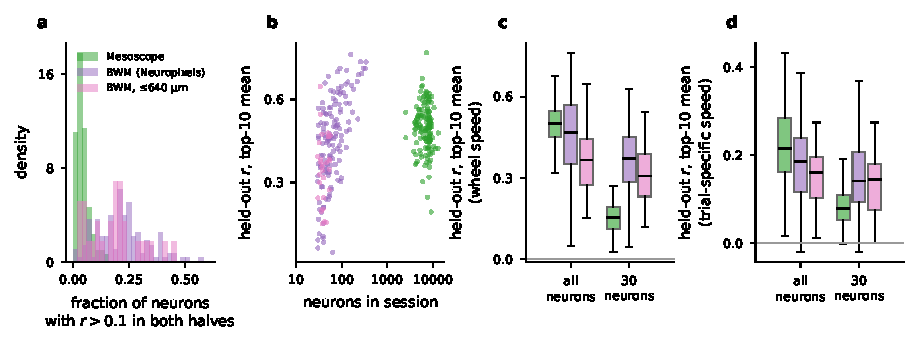
\includegraphics[width=\linewidth,height=0.8\textheight,keepaspectratio]{figures/population.pdf}
  \caption{Wheel-speed correlates are rare in the mesoscope but present: among thousands of neurons per session the best 10 track wheel speed in held-out trials as well as the best BWM units, but a random set of 30 neurons, as in a small spatial bin, contains far fewer of them than a BWM set of the same size. Sessions with $\geq$30 neurons and $\geq$50 trials. \textbf{a} Fraction of neurons per session whose correlation with wheel speed (over all wheel bins) exceeds 0.1 in both the even and the odd trials: median 3.6\% (mesoscope, 149 sessions), 21.7\% (BWM isocortex, 137), 18.2\% (BWM units within 640\,$\mu$m of the surface, 29). \textbf{b} Correlation with wheel speed in the odd trials of the mean z-scored activity of the 10 neurons that correlate best on the even trials, against the number of neurons in the session (one dot per session). \textbf{c} The same with all neurons of a session (median mesoscope 0.50, BWM 0.47, $p$ = 0.03) and with sessions subsampled to 30 random neurons (mean over 20 draws; 0.15 vs 0.37, $p<10^{-32}$). Boxes: quartiles; whiskers: 1.5 inter-quartile ranges. \textbf{d} Same against trial-specific speed (wheel speed minus its per-bin mean over the even trials): 0.22 vs 0.19 (all neurons), 0.08 vs 0.14 (30 neurons).}
  \label{fig:population}
\end{figure}
